Tijekom biološke reprodukcije, genetski materijal roditelja rekombinira se na takav način da se određeni geni prenose na otprilike jednako mjesto unutar kromosoma kao što su bili smješteni unutar onog roditeljskog. Ovo se konceptualno razlikuje od načina jednostavnog križanja, gdje je moguće pomicanje podstabala na potpuno drugačiju poziciju od one izvorišne.

Operatori križanja koji čuvaju poziciju genetskog materijala nazivaju se homolognima. Ovaj operator predstavlja jednu inačicu homolognog križanja i razlikuje se od kasnije spomenutog homolognog operatora križanja. Ovakvi operatori češće su korišteni u linearnom genetskom programiranju gdje je pojam homologije puno intuitivniji i uočljiviji, za razliku od stabala gdje se homolognost može interpretirati na više različitih načina. Posljedično višestrukoj interpretaciji homologije unutar stabala postoji i više vrsta homolognih operatora križanja. 

\begin{figure}[H]
 	\centering


\begin{tikzpicture}
	[sibling distance=25mm, level distance=15mm,
	every node/.style={fill=blue!20,circle,draw,drop shadow, minimum height=1cm}]

\begin{scope}[xshift=0cm]

	\node  [fill=yellow!20]  {\textbf{+}}
    		child {node [fill=yellow!20]  {$cos$}
    			child {node  [fill=yellow!20] {-}
    				child {node{x}}
    				child {node{y}}
    			}
    		}
    		child {node [fill=yellow!20]  {\textbf{$\cdot$}}
        		child {node [fill=yellow!20]  {2}}
        		child {node [fill=yellow!20]  {y}}
      		};
	};
\end{scope}

\begin{scope}[xshift=7cm]
	\node  [fill=yellow!20]  {\textbf{+}}
    		child {node  [fill=yellow!20] {$sin$}
        		child {node  [fill=yellow!20] {y}}
      		}
    		child {node [fill=yellow!20] {\textbf{$/$}}
			child {node [fill=yellow!20]  {x}}
			child {node [fill=yellow!20]  {y}}	
		};
	};
\end{scope}

\end{tikzpicture}


	\caption{Zajedničko područje dva roditelja}
	\label{crxOnePointCommon}
\end{figure}

Križanje s jednom točkom prekida predstavljeno je u \cite{crxOnePoint}, te je prvo križanje koje uzima u obzir homologiju gena. Temelji se na odabiru zajedničke točke križanja unutar roditelja. Pri tome, zajednička točka križanja može se odabrati samo unutar zajedničkih područja roditelja - područja u kojima podstabla oba roditelja imaju potpuno jednak oblik. Primjer zajedničkih područja dan je na slici \ref{crxOnePointCommon}, gdje je zajedničko područje dva roditelja označen žutom bojom. Zajednička područja odgovaraju homologiji u smislu da je velika vjerojatnost da podstabla jednakih oblika obavljaju jednaku ili sličnu funkciju. Također, budući da su podstabla jednakog oblika, pozicija određenog gena je intuitivna i jednoznačna.

Na slici \ref{crxOnePoint} prikazan je rezultat križanja roditelja sa slike \ref{crxOnePointCommon}, gdje je za točku prekida odabran čvor $cos$ unutar prvog, odnosno $sin$ unutar drugog roditelja. 

\begin{figure}[H]
 	\centering


\begin{tikzpicture}
	[sibling distance=25mm, level distance=15mm,
	every node/.style={fill=blue!20,circle,draw,drop shadow, minimum height=1cm}]

\begin{scope}[xshift=0cm]

	\node {\textbf{+}}
    		child {node [fill=red!20]  {$sin$}
    				child {node [fill=red!20]{y}}
    		}
    		child {node {\textbf{$\cdot$}}
        		child {node{2}}
        		child {node {y}}
      		};
	};
\end{scope}

\begin{scope}[xshift=7cm]
	\node   {\textbf{+}}
    		child {node [fill=red!20] {$cos$}
    			child {node [fill=red!20]{-}
    				child {node [fill=red!20]{x}}
    				child {node [fill=red!20]{y}}
    			}
    		}
    		child {node {\textbf{$/$}}
			child {node  {x}}
			child {node  {y}}	
		};
	};
\end{scope}

\end{tikzpicture}


	\caption{Rezultat križanja roditelja sa slike \ref{crxOnePointCommon}}
	\label{crxOnePoint}
\end{figure}

\subsection{Dosadašnji rezultati}

U \cite{onePointExp} provedeno je istraživanje o učinkovitosti ovog operatora nad $n$-paritetnim problemom \footnote{rješenje ovog problema je pronaći funkciju $n$ varijabli koja je za parni broj istinitih varijabli istinita}, za $n$ = 3, 4. Na slici \ref{even3par} prikazani su rezultati za rješavanje 3-paritetnog problema. Ovdje, stupac \textit{Depth } označava dubinu dobivenog rješenja, \textit{$p_m$}  vjerojatnost mutacije, te je u ostalim stupcima prikazan napor uložen u izgradnju točnog rješenja s veličinom jedinke u zagradi. Analogno ovome u \ref{even4par} prikazan je jednak scenarij za 4-paritetni problem.

Na slikama je vidljivo kako ovo križanje u prosjeku daje dosta manja rješenja od jednostavnog križanja, no da je do takvih rješenja nešto teže doći. Ovime se može reći kako ovo križanje ima prednost nad jednostavnim križanjem - brzina pronalaska konačnog rješenja u genetskom programiranju ionako nije jedan od bitnih faktora koji ukazuje na uspješnost samog algoritma.

 \begin{figure}[H]
	\centering
	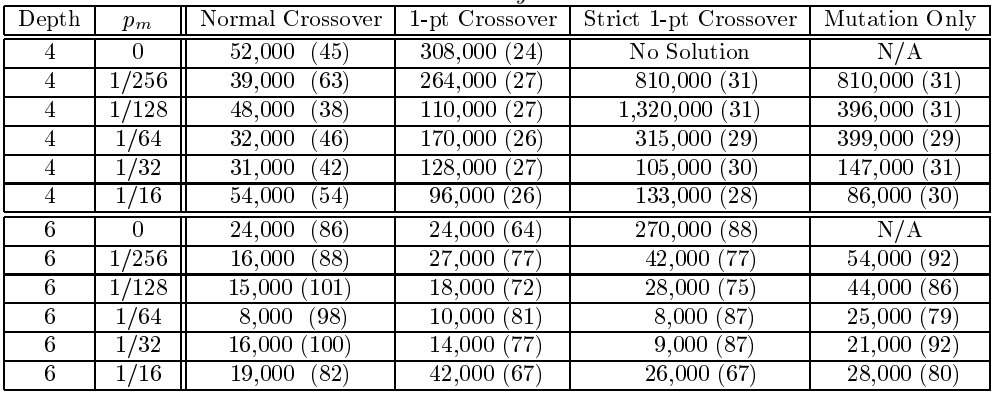
\includegraphics[scale=0.4]{./slike/even3par.png}
	\caption{Rezultati rješavanja 3-paritetnog problema (preuzeto iz \cite{onePointExp})}
	\label{even3par}
\end{figure}

 \begin{figure}[H]
	\centering
	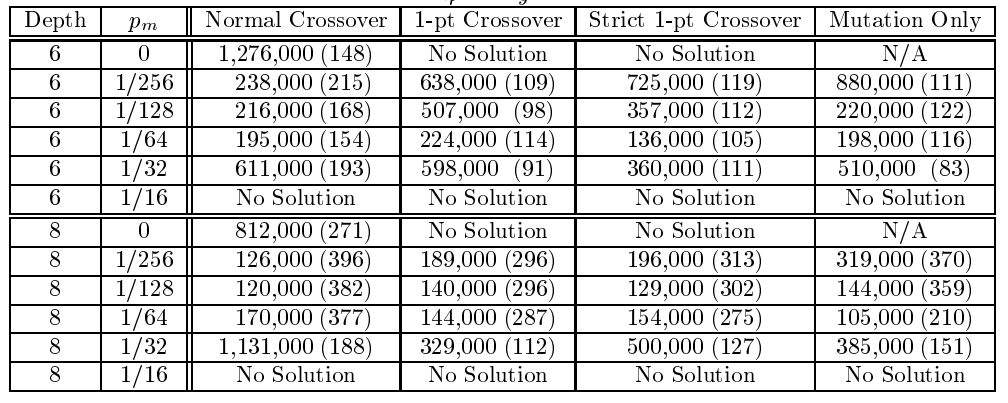
\includegraphics[scale=0.4]{./slike/even4par.png}
	\caption{Rezultati rješavanja 4-paritetnog problema (preuzeto iz \cite{onePointExp})}
	\label{even4par}
\end{figure}
